In the process of developing a machine learning model, 
various artifacts beyond source code are produced. An 
artifact refers to any file that serves as an input or 
output of a given process. In traditional software 
development, inputs such as source code and libraries 
qualify as artifacts, while outputs like object files 
and executables are also considered artifacts. For 
instance, in a build process, these outputs represent 
the results of transforming inputs through the 
compilation pipeline. \cite{wandb, pulicharla2024data}

In the context of machine learning, the most critical 
artifacts are datasets and models. Datasets act as the 
inputs to the training process, while models, which 
encapsulate learned parameters and structures, serve as 
the outputs of this process. \cite{pulicharla2024data}
\begin{figure}[H]
    \centering
    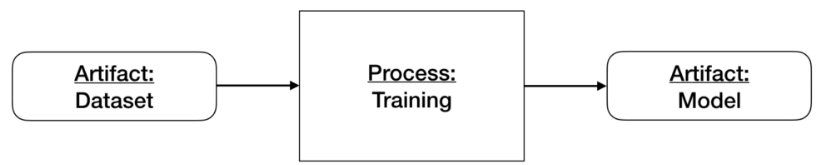
\includegraphics[width=0.8\textwidth]{fig/ml-artifacts.png}
    \caption{Artifacts in Machine Learning \cite{wandb}}
    \label{fig:ml-artifacts}
\end{figure}

\subsection{Use of Data Versioning in Machine Learning}


In machine learning workflows, managing datasets is crucial 
for reproducibility and collaboration. A systematic data 
versioning approach allows teams to track, store, retrieve, 
and switch between dataset versions, ensuring consistency 
across development and experimentation phases. 
\cite{wandb, pulicharla2024data}

The process begins by versioning the dataset, similar to 
tracking changes in source code. Metadata files store 
information about each dataset version, keeping the 
repository efficient while pointing to specific dataset 
versions used in different pipeline stages. 
\cite{pulicharla2024data, opendatascience}

The actual dataset is stored separately, either locally or 
in the cloud, to avoid bloating the version control system. 
This ensures every dataset version is accounted for without 
overwhelming the repository. \cite{opendatascience}

Retrieving a specific dataset version is possible through 
metadata, ensuring reproducibility by matching data with 
the state of the code and experiments. 
\cite{opendatascience, yizhenzhao}

The ability to switch between dataset versions allows 
flexibility during development, supporting iterative testing, 
analysis, and debugging, ensuring synchronization between 
code and data. \cite{opendatascience, yizhenzhao}

Implementing data versioning practices ensures machine 
learning workflows are robust, efficient, and collaborative, 
facilitating seamless transitions through different stages 
of development and research. 
\cite{wandb, opendatascience, yizhenzhao}

\begin{figure}[H]
    \centering
    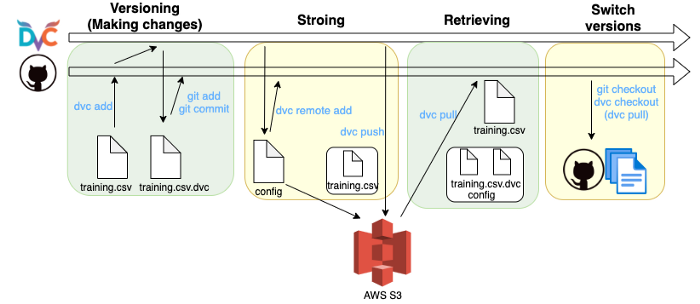
\includegraphics[width=0.8\textwidth]{fig/ml-dv-example.png}
    \caption{Example of how can be data versioning used in 
    machine learning (DVC and GIT as examples) \cite{opendatascience}}
    \label{fig:ml-dv-example}
\end{figure}

\subsection{Advantages of Data Versioning in Machine Learning}

Data versioning in machine learning workflows goes beyond 
tracking changes; it promotes collaboration across teams and 
ensures consistency in model development. By structuring 
versioning, practitioners can manage datasets and models at 
different stages, enabling seamless integration, testing, and 
pipeline improvement. \cite{wandb, opendatascience}
\\\\
It allows branching and merging of datasets, akin to code 
branching in software development. Teams can modify 
foundational datasets for specific needs, organizing changes 
into separate versions while maintaining links to the original 
data. \cite{wandb, opendatascience}
\\\\
Versioning supports "harvesting," where improvements in one 
branch can integrate back into the main dataset or other 
streams, benefiting broader workflows without disrupting 
progress. It also ensures consistency by propagating changes 
across projects. \cite{opendatascience, aimultiple}
\\\\
Hierarchical versioning tracks streams from enterprise-level 
to individual workflows, enabling scalability and evolution 
alongside machine learning models.
\cite{opendatascience, aimultiple}
\\\\
A robust versioning framework ensures data lineage, 
collaboration, and reproducibility, enhancing confidence in 
building, testing, and deploying models.
\cite{opendatascience, aimultiple}

\begin{figure}[H]
    \centering
    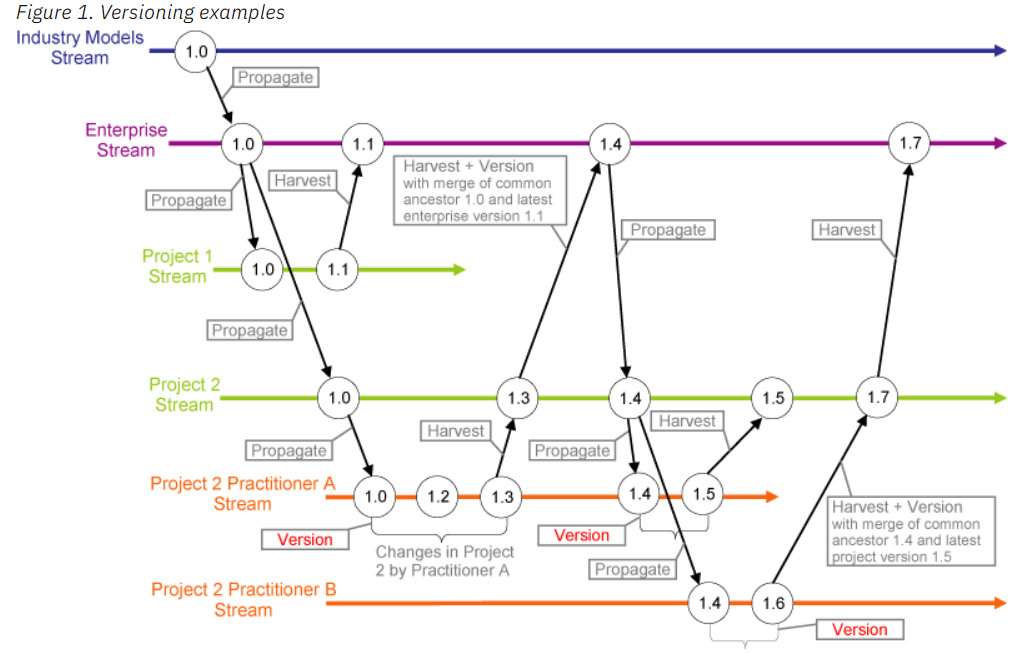
\includegraphics[width=0.8\textwidth]{fig/dv-advantages.png}
    \caption{An example of hierarchical data versioning 
        streams showcasing branching, propagation, and 
        merging across industry, enterprise, project, and 
        individual practitioner levels, enabling collaborative 
        and scalable data management in machine learning 
        workflows \cite{aimultiple}}
    \label{fig:dv-advantages}
\end{figure}
